\documentclass[tikz,convert={outext=.png}]{standalone}
\begin{document}
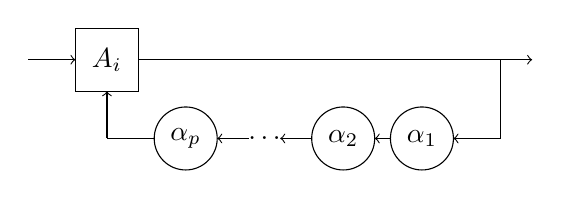
\begin{tikzpicture}[scale=0.2]
\tikzstyle{every node}+=[inner sep=0pt]
\draw [black, ->] (-5,0) -- (-2,0);
\draw [black] (-2,-2) -- (+2,-2) -- (+2,+2) -- (-2,+2) -- cycle;
\draw [black] (0,0) node {$A_i$};
\draw [black, <-] (0,-2) -- (0,-5);

\draw [black, ->] (+2,0) -- (+27,0);

\draw [black] (0,-5) -- (3,-5);

\draw [black] (5,-5) circle (2);
\draw [black] (5,-5) node {$\alpha_p$};

\draw [black, <-] (7,-5) -- (9,-5);

\draw [black] (10,-5) node {$\ldots$};

\draw [black, <-] (11,-5) -- (13,-5);

\draw [black] (15,-5) circle (2);
\draw [black] (15,-5) node {$\alpha_2$};

\draw [black, <-] (17,-5) -- (18,-5);

\draw [black] (20,-5) circle (2);
\draw [black] (20,-5) node {$\alpha_1$};

\draw [black, <-] (22,-5) -- (25,-5);

\draw [black] (+25,0) -- (+25,-5);
\end{tikzpicture}
\end{document}
